\chapter{Normalization Layers}
La normalizzazione è una tecnica cruciale nell’addestramento di reti neurali profonde. Essa viene introdotta per migliorare l’ottimizzazione e stabilizzare l'apprendimento. In particolare, si fa riferimento alla \textbf{Batch Normalization (BN)} come metodo per affrontare problemi legati al cosiddetto \textit{internal covariate shift}.

\section{Covariate Shift}
Il \textbf{Covariate Shift} rappresenta un cambiamento nella distribuzione degli input tra il training e il test. Nelle CNN \textit{(Convolutional Neural Network)} (che vedremo nel capitolo successivo), i cambiamenti nei pesi degli strati inferiori modificano la distribuzione degli input per gli strati successivi, rallentandone pertanto l'addestramento. Questo fenomeno è noto come \textit{internal covariate shift}, vi è un vero e proprio problema, legato al fatto che ci si deve continuamente adattare a nuove distribuzioni, e questa cosa inevitabilmente non farà che rallentarne la convergenza.

\subsection{Problemi di Ottimizzazione}
La BN normalizza gli input degli strati intermedi, imitando un \textit{whitening} (decorrelazione con media zero e varianza unitaria). 
Questo processo è simile alla normalizzazione iniziale degli input delle reti, ma applicato a ogni batch durante l’addestramento.

\subsection{Perché il metodo classico non funziona}
Un approccio classico, ossia allenare una rete e successivamente effettuare la normalizzazione, porta a fallire. Questo poiché la normalizzazione effettuata post hoc, non fa altro che rompere il flusso del gradiente portando a bias esplosivi. La disconnessione fra ottimizzazione e normalizzazione causa dei problemi, per esempio il gradinete non tiene contro dell'effetto della normalizzazione. Pertanto una soluzione proposta è quella di inserire un layer di normalizzazione (Figura~\ref{fig:bn-layer}) all'interno del modello, in questo modo il gradiente lo "vede" e può essere in grado di correggere i parametri della rete in maniera coerente.
\begin{figure}
    \centering
    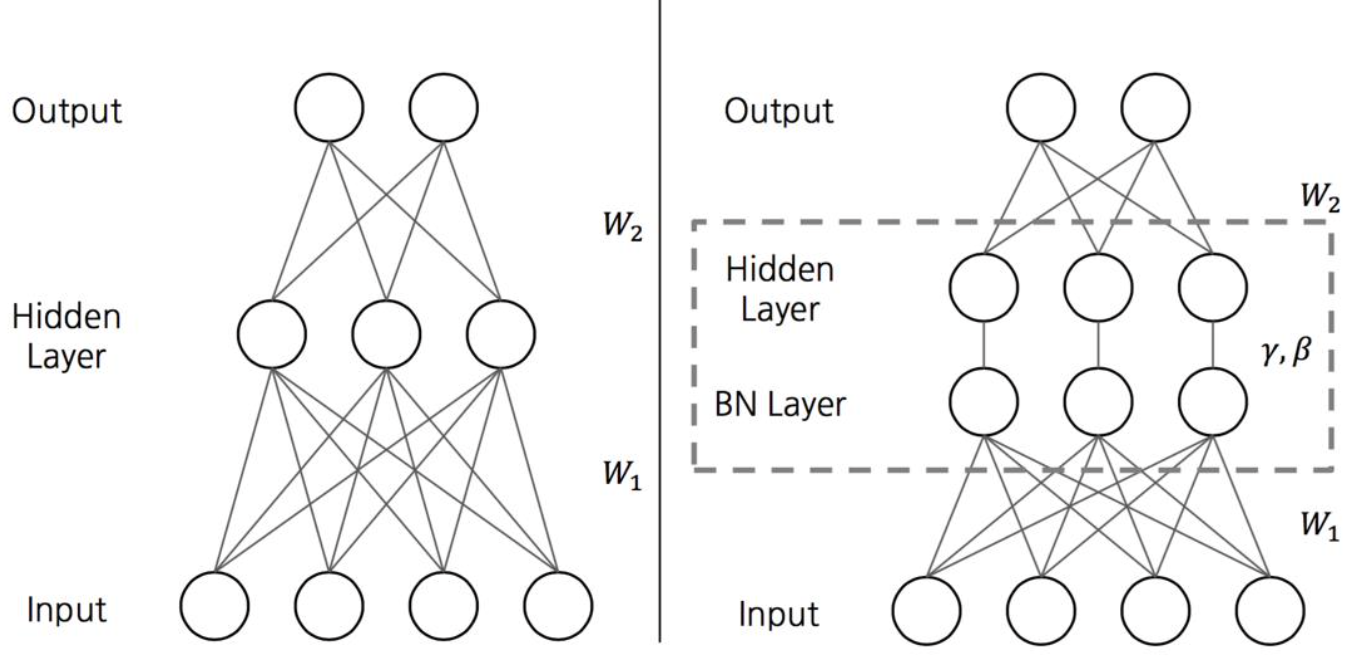
\includegraphics[width=0.85\linewidth]{figure/BNlayer.png}
    \caption{Inserimento di un layer utilizzando la Batch Normalization}
    \label{fig:bn-layer}
\end{figure}
\begin{quote}
“Il layer BN può imparare anche l’identità, rendendo reversibile la normalizzazione se necessario.”
\end{quote}

Analiziamo passo passo, quali sono i passaggi effettuati per giungere a ciò che ottimizza al meglio la Normalizzazione:
\begin{itemize}
  \item Ogni feature è normalizzata separatamente;
  \item Si usa la normalizzazione Z-score;
  \item Le stime di media e varianza vengono calcolate sul batch;
  \item Sono presenti due parametri appresi: $\gamma$ (scaling) e $\beta$ (bias), per mantenere la capacità rappresentativa.
\end{itemize}

Sia $x$ un input, $x^{(k)}$ la $k$-esima feature:

\begin{equation*}
    \mu^{(k)} = \frac{1}{m} \sum_{i=1}^m x_i^{(k)} \quad\quad \sigma^{2(k)} = \frac{1}{m} \sum_{i=1}^m (x_i^{(k)} - \mu^{(k)})^2
\end{equation*}
\begin{equation*}
    \hat{x}_i^{(k)} = \frac{x_i^{(k)} - \mu^{(k)}}{\sqrt{\sigma^{2(k)} + \epsilon}} \quad\quad y_i^{(k)} = \gamma^{(k)} \hat{x}_i^{(k)} + \beta^{(k)}
\end{equation*}

Se non ci fossero i due parametri $\beta$ e $\gamma$ la distribuzione dei valori di output, avrebbe una media nulla e una varianza unitaria e questa cosa non sarebbe utile, pertanto questi due valori non fanno altro che mantenere la forza rappresentativa della rete neurale complessiva.


\subsubsection{Perché la Batch Normalization è efficace}
\begin{itemize}
  \item Rende più stabili le distribuzioni di attivazione;
  \item Riduce l’effetto di gradienti esplosivi/vanescenti;
  \item Permette l’uso di learning rate più alti;
  \item Consente di usare attivazioni sature (e.g. sigmoid);
  \item Diminuisce la necessità di tecniche di regularizzazione;
  \item Riduce il tempo di training;
  \item Migliora la generalizzazione;
  \item Aumenta l'accuratezza.
\end{itemize}

Esistono inoltre varie tipologie di normalizzazione ed essi differiscono semplicemente per la dimensione del gruppo di campioni usati per la normalizzazione, per esempio lungo i canali, i batch presi in considerazioni o ancora la scelta di un singolo esempio.


\subsection{Conclusioni}
Sebbene la normalizzazione funzioni bene nella pratica, le ragioni della sua efficacia sono ancora controverse. In origine, la normalizzazione è stata proposta per ridurre il "Covariate Shift", ma alcuni studiosi hanno dimostrato che questa possibilità non avviene, attraverso degli esperimenti. Tuttavia, la normalizzazione è chiaramente una combinazione dei seguenti fattori:

\begin{itemize}
    \item Le reti con strati di normalizzazione sono più facili da ottimizzare, consentendo l'uso di tassi di apprendimento più elevati;
    \item La normalizzazione ha un effetto di ottimizzazione che accelera l'addestramento delle reti neurali;
    \item Le stime di media e deviazione standard, sono rumorose a causa della casualità dei campioni nel batch. Questo rumore extra si traduce in una migliore generalizzazione in alcuni casi. La normalizzazione ha un effetto di regolarizzazione;
    \item La normalizzazione riduce la sensibilità all'inizializzazione del peso.
\end{itemize}

Di conseguenza, la normalizzazione consente di essere più tranquilli: dando la possibilità di combinare quasi tutti i possibili blocchi di una rete neurale qualsiasi, avendo la possibilità di addestrarne una senza dover considerare quanto essa possa essere mal condizionata.